%****************************************************************************%
%* DIET User's Manual plugin scheduler chapter file                         *%
%*                                                                          *%
%*  Author(s):                                                              *%
%*    - Alan SU (Alan.SU@ens-lyon.fr)                                       *%
%*                                                                          *%
%* $LICENSE$                                                                *%
%****************************************************************************%

%%%%%%%%%%%%%%%%%%%%%%%%%%%%%%%%%%%%%%%%
%% \documentclass{article}

\newenvironment{code}
{\begin{list}{}{\setlength{\leftmargin}{1em}}\item\bfseries\tt}
{\end{list}}

\newenvironment{tinycode}
{\begin{list}{}{\setlength{\leftmargin}{1em}}\item\tiny\bfseries\tt}
{\end{list}}

%% \begin{document}
%%%%%%%%%%%%%%%%%%%%%%%%%%%%%%%%%%%%%%%%

\chapter{Scheduling in \diet}
\label{ch:plugin}

\section{Introduction}

We introduce a \emph{plugin scheduling} facility, designed to allow
\diet service developers to define application-specific performance
measures and to implement corresponding scheduling strategies.  This
section describes the default scheduling policy in \diet and the
interface to the plugin scheduling facility.

\section{Default Scheduling Strategy}\label{sect:default_sched}

The \diet scheduling subsystem is based on the notion that, for the
sake of system efficacy and scalability, the work of determining the
appropriate schedule for a parallel workload should be distributed
across the computational platform.  When a task in such a parallel
workload is submitted to the system for processing, each Server Daemon
(\sed) provides a \emph{performance estimate}~-- a collection of data
pertaining to the capabilities of a particular server in the context
of a particular client request~-- for that task.  These estimates are
passed to the server's parent agent; agents then sort these responses
in a manner that optimizes certain performance criteria.  Effectively,
candidate {\sed}s are identified through a distributed scheduling
algorithm based on pairwise comparisons between these performance
estimations; upon receiving server responses from its children, each
agent performs a local scheduling operation called \emph{server
response aggregation}.  The end result of the agent's aggregation
phase is a list of server responses (from servers in the subtree
rooted at said agent), sorted according to the aggregation method in
effect.  By default, the aggregation phase implements the following
ordered sequence of tests:

\begin{enumerate}
\item \textbf{FAST/NWS data}: {\sed}s compiled and properly configured
  with FAST~\cite{Qui02} and NWS~\cite{WSH99} are capable of making
  dynamic performance estimates.  If such data were generated by the
  {\sed}s, these are the metrics on which agents select servers.
\item \textbf{Round-robin}: In the absence of application- and
  platform-specific performance data, the \diet scheduler attempts to
  probabilistically achieve load balance by assigning client requests
  on a round-robin basis.  Essentially each server records a timestamp
  indicating the last time at which it was assigned a job for
  execution.  Each time a request is received, the \sed computes the
  time elapsed since its last execution, and among the responses it
  receives, \diet agents select {\sed}s with a longer elapsed time.
\item \textbf{Random}: If the {\sed} is unable to store timestamps, the
  \diet scheduler will chose randomly when comparing two otherwise
  equivalent {\sed} performance estimations.
\end{enumerate}

\textbf{Warning:} If \diet is compiled with option \texttt{DIET\_USE\_CORI},
FAST/NWS Scheduling is deactivated (See
Chapter~\ref{chapter:performance} for more information about CoRI).

In principle, this scheduling policy prioritizes servers that are able
to provide useful performance prediction information (as provided by
the FAST and NWS facilities).  In general, this approach works well
when all servers in a given \diet hierarchy are capable of making such
estimations.  However, in platforms composed of {\sed}s with varying
capabilities, load imbalances may occur: since \diet systematically
prioritizes server responses containing FAST and/or NWS data, servers
that do not respond with such performance data will never be
chosen.

We have designed a plugin scheduler facility to
enable the application developer to tailor the \diet scheduling to the
targeted application.
This functionality provides
the application developer the means to extend the notion of a
performance estimation to include metrics that are
application-specific, and to instruct \diet how to treat those data in
the aggregation phase.
We describe these interfaces in the following sections.


\section{Plugin Scheduler Interface}

Distributed applications are varied and often exhibit performance
behavior specific to the domain from which they arise.  Consequently,
application-specific scheduling approaches are often necessary to
achieve high-performance execution.  We propose an extensible
framework to build
\emph{plugin schedulers}, enabling application developers to specify
performance estimation metrics that are tailored to their individual
needs.

%% This section introduces the principal components of the basic plugin
%% scheduler framework.

\subsection{Estimation Metric Vector}\label{sect:estvector}

The new type \texttt{estVector\_t} represents an
\emph{estimation vector}, logically a structure that can manage a
dynamic collection of performance estimation values.  It contains
values that represent the performance profile provided by a
{\sed} in response to a \diet service request.  This collection of values
may include either standard performance measures that are available
through \diet, or developer-defined values that are meaningful solely in
the context of the application being developed.

\subsection{Standard Estimation Tags}\label{sect:estTags}

To access to the different fields of the \texttt{estVector\_t}, it is
necessary to specify the tag that correspond to a specific information
type.  Table~\ref{t:tags} describes this correspondence.  Some tags
represent a list of values, one has to use the
\texttt{diet\_est\_array\_*}  functions to have access to them. In
Table~\ref{t:tags},  the second column marks these multi-value tags.

The tag \textit{ALLINFOS} is a special: his field is 
always empty, but it allows to fill the vector with all known tags 
by the particular collector.
 
\begin{table}[h]
 \tiny
 \centering
 \begin{tabular}[c]{|c|c|c|}\hline
%FAST ligne

  \texttt{Information tag}  &multi-& \texttt{Explication} \\[5pt]
 \texttt{starts with EST\_} &value& \\[5pt]
  \hline

%TAGS lines
 \textit{TCOMP        }&& the predicted time 
                       to solve a problem \\[5pt]
  \hline
  \textit{TIMESINCELASTSOLVE} &   & time since last solve has been made (sec) \\[5pt]
  \hline
  \textit{FREECPU      }&& amount of free CPU power between 0 and 1 \\[5pt]
  \hline
  \textit{FREEMEM      }&& amount of free  memory (Mb) \\[5pt]
  \hline
  \textit{NBCPU        }&& number of available processors  \\[5pt]
  \hline
  \textit{CPUSPEED     }&x& frequency of CPUs (MHz) \\[5pt]
  \hline
  \textit{TOTALMEM     }&& total memory size (Mb)  \\[5pt]
  \hline
  \textit{AVGFREECPU   }&& average amount of free CPU power in [0..1] \\[5pt]
  \hline
  \textit{BOGOMIPS     }&x& CPUs' bogomips \\[5pt]
  \hline
  \textit{CACHECPU     }&x& cache size CPUs (Kb) \\[5pt]
  \hline
  \textit{TOTALSIZEDISK}&& size of the partition (Mb)\\[5pt]
  \hline
  \textit{FREESIZEDISK }&& amount of free place on partition (Mb)\\[5pt]
  \hline
  \textit{DISKACCESREAD}&& average time to read on disk (Mb/sec) \\[5pt]
  \hline
  \textit{DISKACCESWRITE}&& average time to write to disk (sec) \\[5pt]
  \hline
  \textit{ALLINFOS     }&x& [empty] fill all possible fields \\[5pt]
  \hline
  \textit{PARAL\_NB\_FREE\_RESOURCES\_IN\_DEFAULT\_QUEUE} & & number
  of idle resources \\[5pt] 
  \hline
 \end{tabular}
 \caption{Explication of the estimation tags}
 \label{t:tags}
\end{table}

\subsubsection{Standard Performance Metrics}

To access to the existing default performance estimation
routines (as described in Chapter~\ref{chapter:performance}), the following
functions are available to facilitate the construction of custom
performance estimation functions:
\begin{itemize}
\item FAST- and NWS-based performance estimation metrics can be used in the plugin scheduler. 
  See the Section~\ref{subsection:callFAST} for information on how to use them.
\item The time elapsed since the last execution (to enable
  the round-robin scheduler) is stored in an estimation metric vector
  by calling
  \begin{tabbing}
    \texttt{int diet\_estimate\_lastexec(}\=\texttt{estVector\_t ev,} \\
    \> \texttt{const diet\_profile\_t* const profilePtr)};
  \end{tabbing}
  with an appropriate value for \texttt{ev} and the
  \texttt{profilePtr} corresponding to the current \diet request.
\item The number of waiting jobs when using the maximum concurrent jobs
  limit is stored in an estimation metric vector by calling
  \begin{tabbing}
    \texttt{int diet\_estimate\_waiting\_jobs(}\=\texttt{estVector\_t ev)};
  \end{tabbing}
\item CoRI allows to access in an easy way to basic performance 
prediction. See Chapter~\ref{sec:CORI} to know more about the use of it.

\end{itemize}

In the future, we plan to expand the suite of default estimation
metrics to include dynamic internal \diet system state information
(\eg queue lengths).

\subsubsection{Developer-defined Performance Metrics}

Application developers may also define performance values to be
included in a \sed response to a client request.  For example, a \diet
\sed that provides a service to query particular databases may need to
include information about which databases are currently resident in
its disk cache, in order that an appropriate server be identified for
each client request.  To store such values, the \sed developer should
first choose a unique integer identifier, referred to as the
\emph{tag} to denote each logical datum to be stored.  Values are
associated with tags using the following interface:
\begin{code}
int diet\_est\_set(estVector\_t ev, int userTag, double value);
\end{code}
The \texttt{ev} parameter is the estimation vector where the
value will be stored, the \texttt{userTag} parameter denotes the
chosen tag, and \texttt{value} indicates the value to be associated
with the tag.  Tagged data are used to effect
scheduling policies by defining custom server response
aggregation methods, described in Section~\ref{sect:agg_methods}.

\subsection{Estimation Function}\label{sect:est_fn}

The default behavior of a {\sed} when a service request arrives from
its parent agent is to store the following information in the
request profile:
\begin{enumerate}
\item \textbf{FAST-based execution time predictions}: \diet {\sed}s
  attempt to call FAST
  routines to obtain execution time predictions based on the type of
  service requested, if FAST was available at compilation time.  If
  available, such predictions are stored in the
  performance estimate.
\item \textbf{NWS-based dynamic resource information}: If NWS library
  functions are available, performance estimates may include dynamic
  resource performance information about CPU availability, free
  memory, and network bandwidth.
\item \textbf{Elapsed time since last execution}: To implement the
  default round-robin behavior in absence of FAST and NWS facilities,
  each {\sed} stores a timestamp of its last execution.  When a service
  request arrives, the difference between that timestamp and the
  current time is added to the performance estimate.
\end{enumerate}
This is accomplished by using the \texttt{diet\_estimate\_fast} and
\texttt{diet\_estimate\_lastexec} functions described in
Section~\ref{sect:estvector}.

To implement a plugin scheduler, we define an
interface that admits customizable performance estimation routines:
\begin{tabbing}
  \texttt{typedef void (* diet\_perfmetric\_t)(}
    \=\texttt{diet\_profile\_t*,} \\
    \>\texttt{estVector\_t);} \\
\end{tabbing}
\begin{tabbing}
  \texttt{diet\_perfmetric\_t} \\
  \texttt{diet\_service\_use\_perfmetric(diet\_perfmetric\_t perfmetric\_fn);}\\
\end{tabbing}
%% \begin{code}
%%   diet\_perfmetric\_t\\
%%   diet\_service\_use\_perfmetric(diet\_perfmetric\_t perfmetric\_fn);\\
%% \end{code}
Thus, the type \texttt{diet\_perfmetric\_t} is a function pointer that
takes as arguments a performance estimation (represented by the
\texttt{estVector\_t} object) and a \diet service request
profile.  The application
developer can associate such a function, or
\emph{performance estimation routine}, with \diet services via the
\texttt{diet\_service\_use\_perfmetric} interface.  This interface
returns the previously registered performance estimation routine, if
one was defined (and
\texttt{NULL} otherwise).  At this point, a service added using the
\texttt{diet\_service\_table\_add} function will be associated with
the declared performance estimation routine.
Additionally, a performance estimation routine so specified will be
associated with \emph{all} services added into the service table until
another call to the
\texttt{diet\_service\_use\_perfmetric} interface is made.
In the performance estimation routine, the {\sed} developer should store
in the provided estimation vector
any performance data used in the server response aggregation
methods (described in the next section).

\subsection{Aggregation Methods}\label{sect:agg_methods}

At the time a \diet service is defined, an \emph{aggregation method}~--
the logical mechanism by which {\sed} responses are sorted~-- is
associated with the service; the default behavior was described in
Section~\ref{sect:default_sched}.

If application-specific data \emph{are} supplied (i.e.,~the
estimation function has been redefined), an alternative method for
aggregation is needed.  Currently, a basic
\emph{priority scheduler} has been implemented, enabling an
application developer to specify a series of performance values that
are to be optimized in succession.  A developer may implement a
priority scheduler using the following interface:
\begin{code}
\begin{tabbing}
diet\_aggregator\_desc\_t* \\
diet\_profile\_desc\_aggregator(diet\_profile\_desc\_t* profile); \\
\\
int diet\_aggregator\_set\_type(\=diet\_aggregator\_desc\_t* agg, \\
\> diet\_aggregator\_type\_t atype); \\
\\
int diet\_aggregator\_priority\_max(\=diet\_aggregator\_desc\_t* agg, \\
\> diet\_est\_tag\_t tag); \\
\\
int diet\_aggregator\_priority\_min(\=diet\_aggregator\_desc\_t* agg, \\
\> diet\_est\_tag\_t tag); \\
\\
int diet\_aggregator\_priority\_maxuser(\=diet\_aggregator\_desc\_t* agg, \\
\> int val); \\
\\
int diet\_aggregator\_priority\_minuser(\=diet\_aggregator\_desc\_t* agg, \\
\> int val); \\
\end{tabbing}
\end{code}
The \texttt{diet\_profile\_desc\_aggregator} and
\texttt{diet\_aggregator\_set\_type} functions fetch and configure the
aggregator corresponding to a \diet service profile, respectively.
In particular, a priority scheduler is declared by invoking the latter
function with \texttt{DIET\_AGG\_PRIORITY} as the \texttt{agg}
parameter.
Recall that from the point of view of an agent, the aggregation phase
is essentially a sorting of the server responses from its children.
A priority scheduler logically uses a series of user-specified tags to
perform the pairwise server comparisons needed to construct the
sorted list of server responses.

To define the tags and the order in which they should be compared,
four functions are introduced.  These functions, of the form
\texttt{diet\_aggregator\_priority\_*}, serve to identify the
estimation values to be optimized during the aggregation phase.  The
\texttt{\_min} and \texttt{\_max} forms indicate that a standard
performance metric (e.g.,~time elapsed since last execution, from the
\texttt{diet\_estimate\_lastexec} function) is to be either
minimized or maximized, respectively.  Similarly, the
\texttt{\_minuser} and \texttt{\_maxuser} forms indicate the analogous
operations on user-supplied estimation values.  Calls to these
functions indicate the order of \textbf{precedence} of the tags.

Each time two server responses need to be compared, the values
associated with the tags specified in the priority aggregator are
retrieved.  In the specified order, pairs of corresponding values are
successively compared, passing to the next tag only if the values for
the current tag are identical.  If one server response contains a
value for the metric currently being compared, and another does not,
the response with a valid value will be selected.  If at any point
during the treatment of tags \emph{both} responses lack the necessary
tag, the comparison is declared indeterminate.
This process continues until one response is
declared superior to the other, or all tags in the priority aggregator
are exhausted (and the responses are judged equivalent).


\section{Example}

A new example has been added to the \diet distribution to illustrate
the usage of the plugin scheduler functionality; this code is
available in the directory
\begin{code}
src/examples/plugin\_example/
\end{code}
A \diet server and client corresponding to a simulation of a
database research application are provided.  If the construction of
examples was enabled during \diet configuration, two binaries
\texttt{server} and \texttt{client} will be built in this directory.
Having deployed a \diet agent hierarchy, the server may be
instantiated:
\begin{code}
  \$ server <SeD\_config> <DB> [ <DB> ... ]
\end{code}
where \texttt{<DB>} are string(s) that represent the existence of
a particular database at the {\sed}'s site.  A client would pose a query
against a set of databases:
\begin{code}
  \$ client <client\_config> <DB> [ <DB> ... ]
\end{code}
The application uses the plugin scheduling facility to prioritize the
existence of databases in selecting a server, and thus, the expected
result is that one of the {\sed}s with the fewest number of database
mismatches will be selected.

In the \texttt{main} function of the \texttt{server.c} file, the
following block of code (a)~specifies the use of the priority
aggregator for this service, (b)~declares a performance estimation
function to supply the necessary data at request-time, and
(c)~defines the order of precedence of the performance values
(i.e.,~minimizing the number of database mismatches, and then
maximizing the elapsed execution time).
\begin{verbatim}
  {
    /* new section of the profile: aggregator */
    diet_aggregator_desc_t *agg;
    agg = diet_profile_desc_aggregator(profile);

    /* for this service, use a priority scheduler */
    diet_aggregator_set_type(agg, DIET_AGG_PRIORITY);          /* (a) */

    /* install our custom performance function */
    diet_service_use_perfmetric(performanceFn);                /* (b) */

    /* define the precedence order */
    diet_aggregator_priority_minuser(agg, 0);                  /* (c) */
    diet_aggregator_priority_max(agg, EST_TIMESINCELASTSOLVE); /* (c) */
  }
\end{verbatim}
The performance function \texttt{performanceFn} is defined as follows:
\begin{verbatim}
static void performanceFn(diet_profile_t* pb, estVector_t perfValues);

[...]

/*
** performanceFn: the performance function to use in the DIET
**   plugin scheduling facility
*/
static void
performanceFn(diet_profile_t* pb, estVector_t perfValues)
{
  const char *target;
  int numMismatch;

  /* string value must be fetched from description; value is NULL */
  target = (diet_paramstring_get_desc(diet_parameter(pb, 0)))->param;
  numMismatch = computeMismatches(target);

  /*
  ** store the mismatch value in the user estimate space,
  ** using tag value 0
  */
  diet_est_set(perfValues, 0, numMismatch);

  /* also store the timestamp since last execution */
  diet_estimate_lastexec(perfValues, pb);
}
\end{verbatim}
The function \texttt{computeMismatches} (defined earlier in
\texttt{server.c}) calculates the number of requested databases that
are not present on the {\sed} making the evaluation.
Together, these two code segments serve to customize the generation of
performance information and the treatment of these data in the context
of the simulated database search.
Finally, it should be noted that the existence of a plugin scheduler
is completely transparent to the client, and thus client code need not
be changed.

%
% Scheduling at agents level
%
%\documentclass{article}

%\usepackage{graphicx}
%\usepackage{fullpage}

%\begin{document}
\section{Scheduler at agents level}
In this section we introduce a new way to define a scheduling policy in DIET.
Some scheduling strategies could not be developed using only the DIET SeDs
plugins. The schedulers at agents level allow the developper to design every
scheduler strategies, even the centralized ones. The two first sections
explain precisely how DIET performs the scheduling. The third section enters
in the DIET source code and can be ignored by most of the users. The
fourth section presents the tools provided to make an agent scheduler
easily. The fifth section treats of the scheduler module compilation and
usage. The last section presents some scheduler examples.
\subsection{Scheduling from the agents side.}
In DIET, the scheduling works as follows (see Figure \ref{scheduleSteps} for
a representation of each step): 
\begin{itemize}
  \item A request is submitted to the Master Agent (step 1).
  \item The Master Agent forwards the request to the Local Agents and SeDs that
    it manages (step 2).
  \item The SeDs which dispose of the asked service return a CORBA response
    structure which contains an estimation metric vector (step 3).
  \item According to a default policy or a user-defined one, the responses
    from the SeDs are aggregated. Then the responses sequence is sent to
    the parent agent which aggregates all the results of its children (step 4).
  \item When the aggregated responses reach the Master Agent, it returns
    the aggregated list of all responses to the client (step 5).
  \item Then, the client chooses the better server, according to the
    chosen aggregation method (step 6).
\end{itemize}
\newlength{\schdlFigWidth}
\setlength{\schdlFigWidth}{(\textwidth - 3mm) / 3}
\begin{figure}[h]
  \centering
  \begin{minipage}{\schdlFigWidth}
    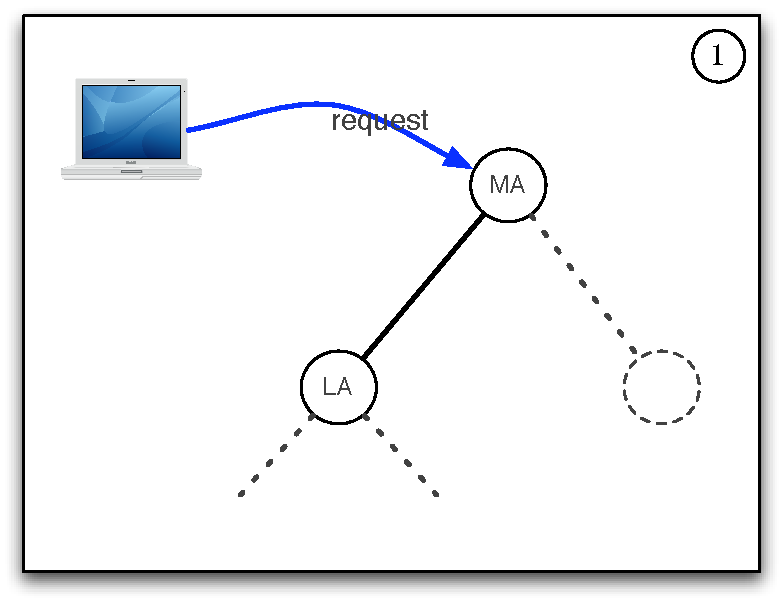
\includegraphics[width=\schdlFigWidth]{fig/schdl00}
  \end{minipage}
  \begin{minipage}{\schdlFigWidth}
    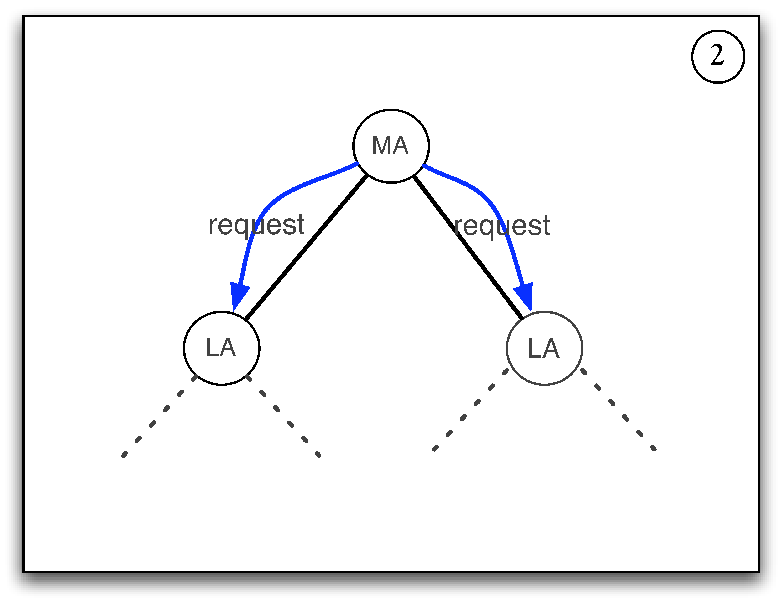
\includegraphics[width=\schdlFigWidth]{fig/schdl01}
  \end{minipage}
  \begin{minipage}{\schdlFigWidth}
    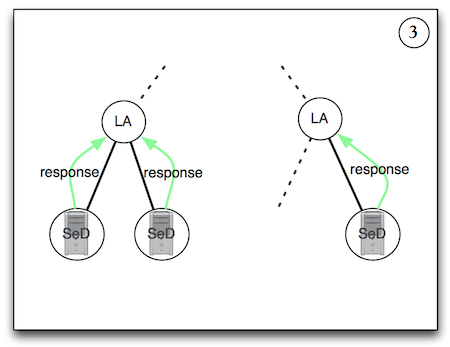
\includegraphics[width=\schdlFigWidth]{fig/schdl02}
  \end{minipage}\\
  \begin{minipage}{\schdlFigWidth}
    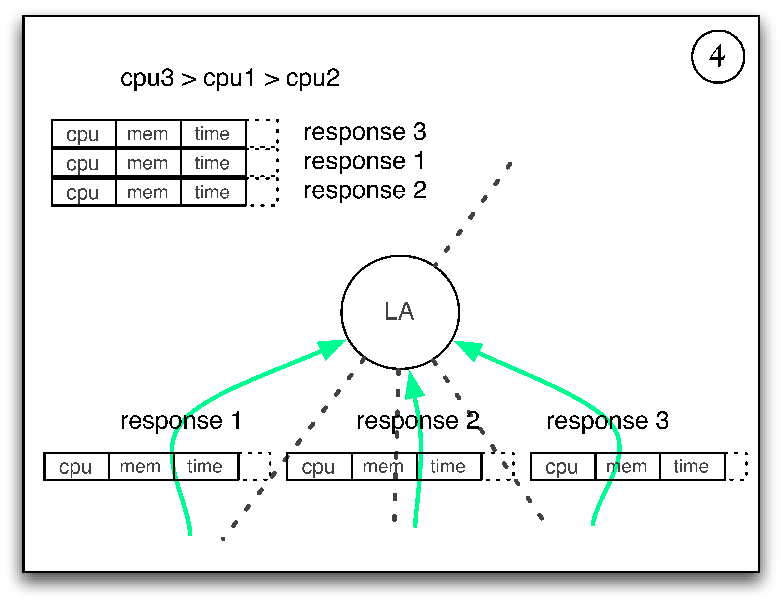
\includegraphics[width=\schdlFigWidth]{fig/schdl03}
  \end{minipage}
  \begin{minipage}{\schdlFigWidth}
    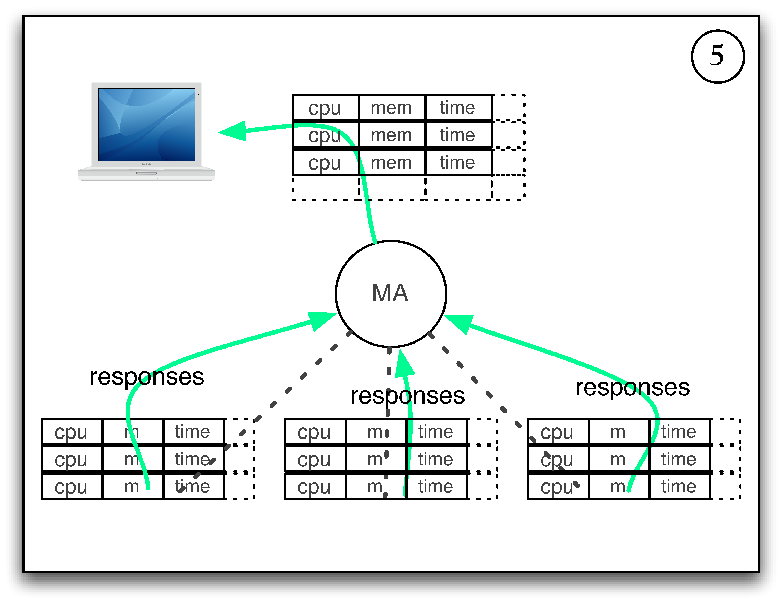
\includegraphics[width=\schdlFigWidth]{fig/schdl04}
  \end{minipage}
  \begin{minipage}{\schdlFigWidth}
    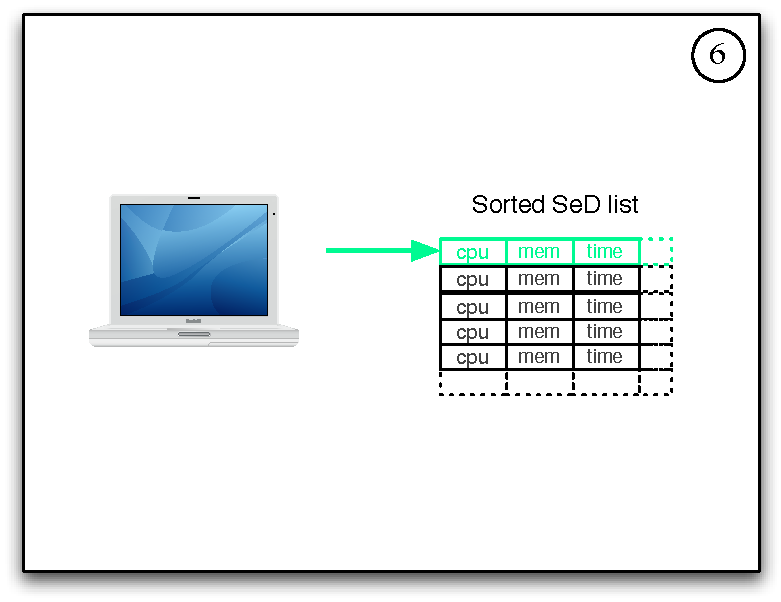
\includegraphics[width=\schdlFigWidth]{fig/schdl05}
  \end{minipage}
  \caption{The steps of the scheduling in DIET.\label{scheduleSteps}}
\end{figure}

\subsection{Aggregation methods overloading}
To aggregate the responses of the SeDs, DIET uses an aggregation method
which is called on the agents. This method is chosen from the SeDs
by defining the aggregator type (see Section \ref{sect:estTags}).
By default, two aggregator types are proposed by DIET:
DIET\_AGG\_DEFAULT and DIET\_AGG\_PRIORITY. In the last versions of DIET, we
introduced a new aggregator type: DIET\_AGG\_USER. Using this
aggregator, the user can define its own aggregation method to be used in
the agents. 
Figure \ref{fig:DIETScheduling} presents the global schedulers classes
organization in DIET. By choosing the DIET\_AGG\_USER aggregator, the user
commands to the GlobalScheduler class to load an external module containing
a UserScheduler class overloading the \textit{aggregate} method.
\begin{figure}[h]
  \centering
  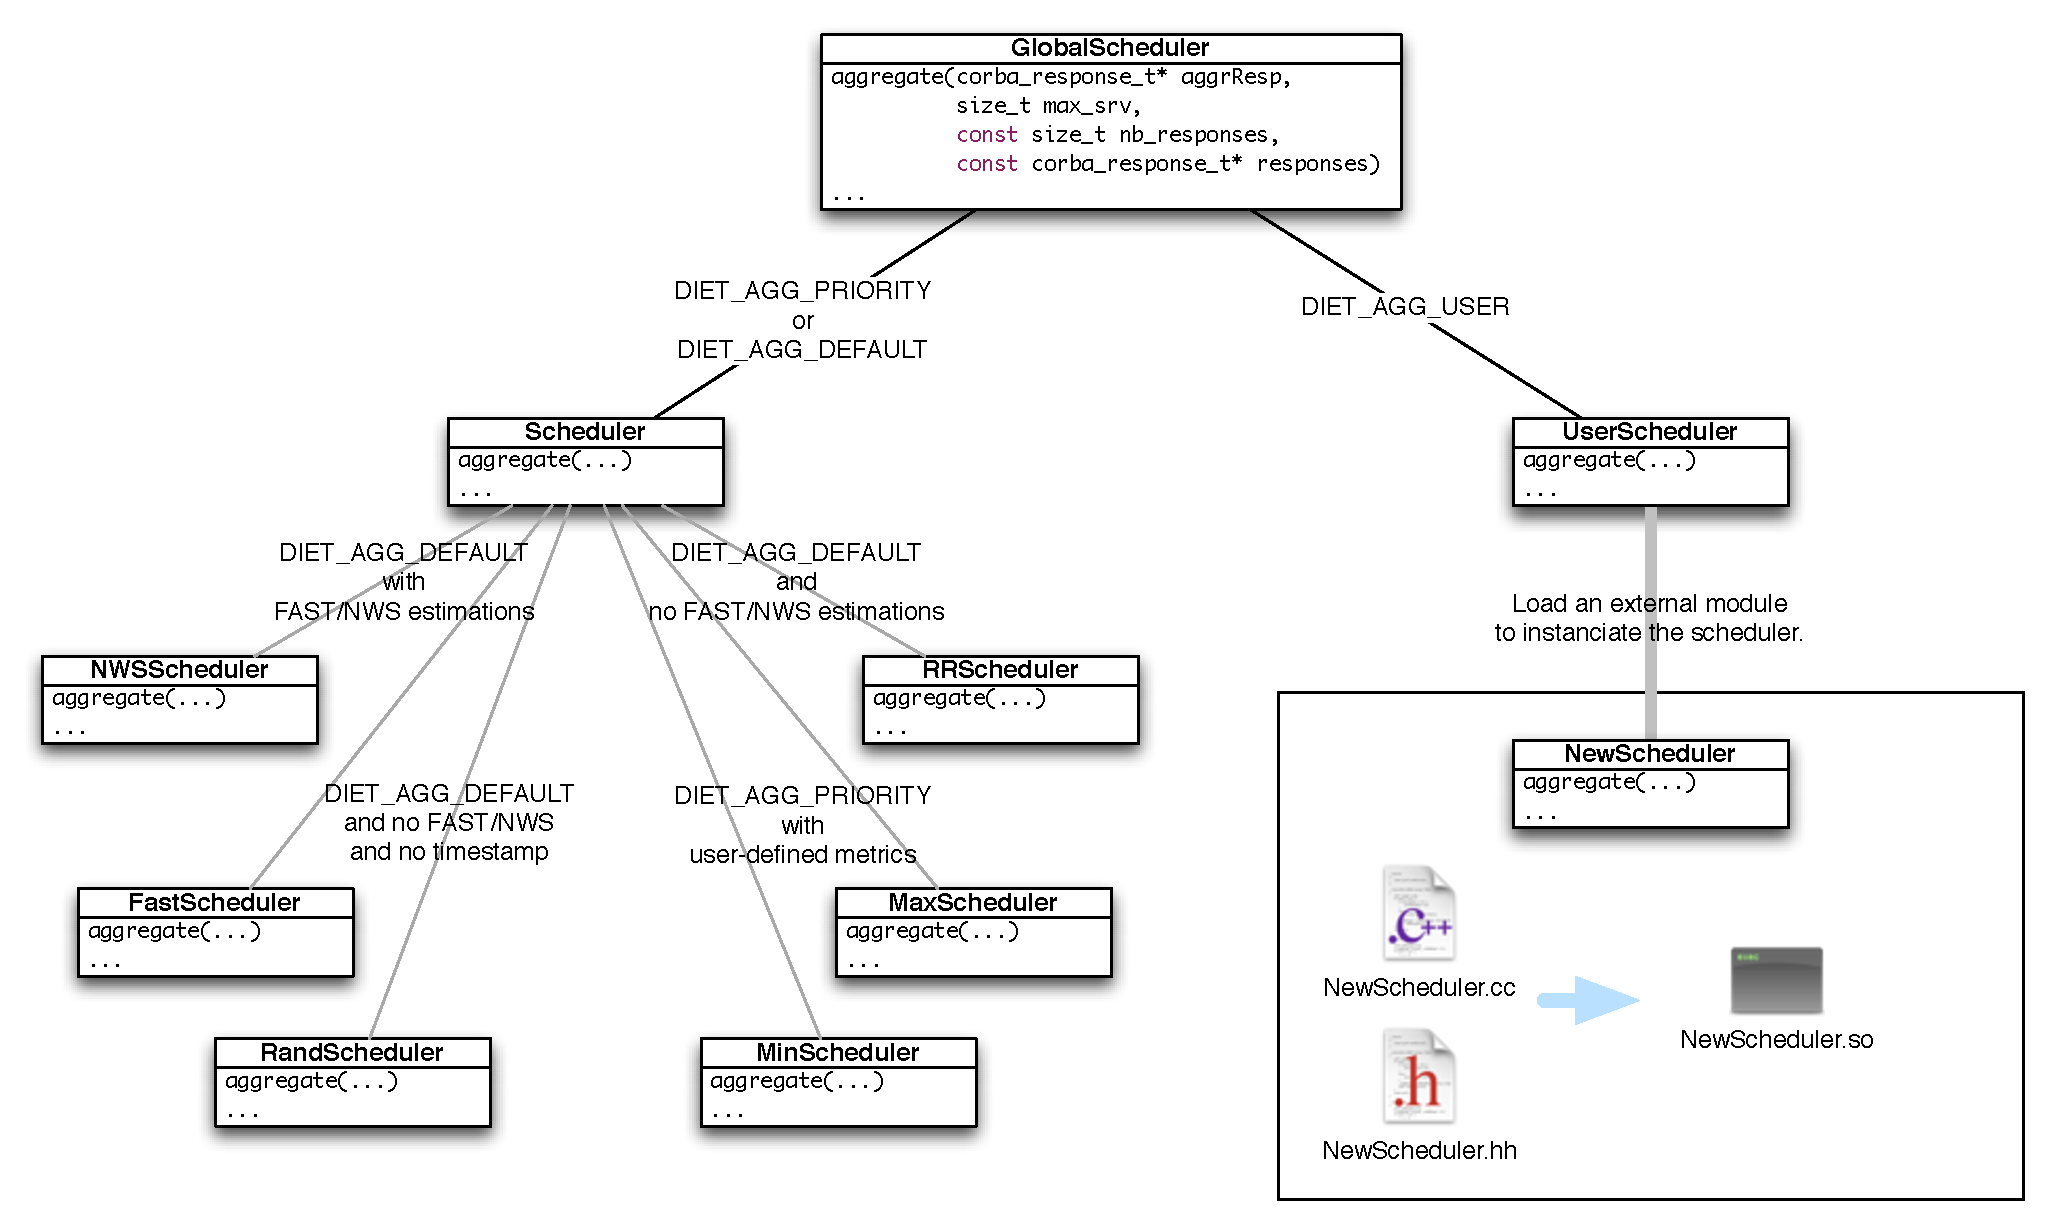
\includegraphics[width=16cm]{fig/DIETScheduling}
  \caption{Schedulers classes organization in DIET.\label{fig:DIETScheduling}}
\end{figure}

The user-defined aggregation method just needs to sort the responses from the
SeDs. By locating the aggregation method on the agent, we can use different
scheduling strategies which could not be implemented at the SeD level. These
schedulers can also avoid some scheduling problems while submitting asynchronous
jobs (with Round-Robin schedulers for example).

\subsection{The UserScheduler class}
This section presents how the scheduling process is managed in DIET.
Most of the developers can go directly to the next section.

All the schedulers developed by users have to inherit from the
\textit{UserScheduler} class. This class furnishes the methods to load
its subclasses as a Scheduler class for DIET without error. The only method
a user has to overload is the \textit{aggregate} method. Several useful
functions and macros are defined in the \textit{UserScheduler.hh} file.
The \textit{UserScheduler} class is defined as below:
\begin{verbatim}
class UserScheduler : public GlobalScheduler
{
  typedef GlobalScheduler* constructor();
  typedef void destructor(UserScheduler*);

public:
  static const char* stName;
  UserScheduler();
  virtual
  ~UserScheduler();
  /** These methods are used to load the user module and to obtain an
     instance of the scheduler. */
  static UserScheduler* getInstance(const char* moduleName);
  static GlobalScheduler * instanciate(const char* moduleName);
  void destroy(GlobalScheduler* scheduler);

  static
  GlobalScheduler* deserialize(const char* serializedScheduler,
			       const char* moduleName);
  static
  char* serialize(GlobalScheduler* GS);
  /** The method that has to be overloaded to define a new scheduler. */
  virtual int
  aggregate(corba_response_t* aggrResp,
            size_t max_srv,
            const size_t nb_responses,
            const corba_response_t* responses);

private:
  /** The UserScheduler class is a singleton class. Its constructor is
   private. */
  UserScheduler(const char* moduleName);
  static UserScheduler* instance;
  void* module;
  /** These two methods are obtained from the loaded module. */
  constructor* constructs;
  destructor* destroys;
};
\end{verbatim}

\noindent The \textit{aggregate} method takes 4 arguments:
\begin{itemize}
  \item \textit{corba\_response\_t* \bf aggrResp}: the result of the aggregation
    has to be set in this argument. \textit{\bf aggrResp} is an array of
    \textit{corba\_server\_estimation\_t} objects. 
  \item \textit{size\_t \bf max\_srv}: this argument gives the maximum number
    of responses to return in \textit{\bf aggrResp}. This value can be ignored
    without any risk and it is sometimes useful to ignore it because this
    parameter is hard-coded in the DIET sources.
  \item \textit{const size\_t \bf nb\_responses}: this argument gives the number
    of responses in \textit{\bf responses}.
  \item \textit{const corba\_response\_t* \bf responses}: the responses are
    stored in this argument. It is an array of \textit{corba\_response\_t}
    which is a CORBA structure containing a CORBA sequence of
    \textit{corba\_server\_estimation\_t}.
\end{itemize}

\noindent The \textit{corba\_response\_t} structure is defined as follows:
\begin{verbatim}
struct corba_response_t {
  typedef _CORBA_ConstrType_Variable_Var<corba_response_t> _var_type;  
  CORBA::ULong reqID;
  CORBA::Long myID;
  SeqServerEstimation_t servers;
  void operator>>= (cdrStream &) const;
  void operator<<= (cdrStream &);
};
\end{verbatim}

\noindent The \textit{\bf \_var\_type} field is an internal CORBA object. The
scheduler developer does not have to use it. The two operators
\textit{\bf operator$>>=$} and \textit{\bf operator$>>=$} can be ignored too.
\begin{itemize}
  \item \textit{CORBA::ULong \bf reqID}: this field contains the ID of the
    request.
  \item \textit{CORBA::Long \bf myID}: this field is for DIET internal usage.
    The developer should ignore it.
  \item \textit{SeqServerEstimation\_t \bf servers}: this field is a sequence
    of \textit{corba\_server\_estimation\_t}. It is used to store the SeDs
    references returned by the \textit{aggregate} method. This is the field
    that has to be sorted/filtered.
\end{itemize}

\noindent The \textit{corba\_server\_estimation\_t} is defined as follows:
\begin{verbatim}
struct corba_server_estimation_t {
  typedef _CORBA_ConstrType_Variable_Var<corba_server_estimation_t> _var_type;
  corba_server_t loc;
  corba_estimation_t estim;
  void operator>>= (cdrStream &) const;
  void operator<<= (cdrStream &);
};
\end{verbatim}
\begin{itemize}
  \item \textit{corba\_server\_t \bf loc}: this field is used to designate a
    particular SeD.
  \item \textit{corba\_estimation\_t estim}: this field contains the estimation
    vector for the designated SeD.
\end{itemize}

\noindent The \textit{corba\_server\_t \bf loc} structure is defined as
follows:
\begin{verbatim}
struct corba_server_t {
  typedef _CORBA_ConstrType_Variable_Var<corba_server_t> _var_type;  
  _CORBA_ObjRef_Member< _objref_SeD, SeD_Helper>  ior;
  CORBA::String_member hostName;
  CORBA::Long port;
  void operator>>= (cdrStream &) const;
  void operator<<= (cdrStream &);
};
\end{verbatim}
The two interesting fields are:
\begin{itemize}
  \item \textit{\bf ior} which is a CORBA reference to the SeD.
  \item \textit{\bf hostName} which is the hostname of the SeD.
\end{itemize}

\noindent The \textit{corba\_estimation\_t} structure is defined as follows:
\begin{verbatim}
struct corba_estimation_t {
  typedef _CORBA_ConstrType_Variable_Var<corba_estimation_t> _var_type;
  SeqEstValue_t estValues;
  void operator>>= (cdrStream &) const;
  void operator<<= (cdrStream &);
};
\end{verbatim}
\textit{SeqEstValue\_t \bf estValues}: This field is a CORBA sequence of
estimation values. These estimation values are accessed through the specific
functions: \textit{diet\_est\_get\_internal} and
\textit{diet\_est\_array\_get\_internal} defined in scheduler/est\_internal.hh.

\noindent These functions prototypes are:
\begin{verbatim}
double diet_est_get_internal(estVectorConst_t ev, int tag, double errVal);
double diet_est_array_get_internal(estVectorConst_t ev, int tag, int idx, double errVal);
\end{verbatim}
\begin{itemize}
  \item \textit{ev}: the estimation vector to evaluate.
  \item \textit{tag}: the estimation tag.
  \item \textit{idx}: the index of the value when available. For example, to
    obtain the frequency of the second processor, we have to set $idx$ to 1.
  \item \textit{errVal}: the value returned by the function if an error
    occurred.
\end{itemize}

\noindent The \textit{tag} argument may be assigned one of the following values:
\begin{itemize}
  % \item EST_TOTALTIME: The total time to execute the request evaluated
  %   by FAST. (FAST must be activated at the compilation time)
  % \item EST_COMMTIME: The communication time evaluated by FAST.
  %   (FAST must be activated at the compilation time)
  \item[-] EST\_TCOMP: The computation time evaluated by FAST
    (FAST must be activated at the compilation time).
  \item[-] EST\_TIMESINCELASTSOLVE: The time elapsed since this SeD solved
    a request. This value is used by the default Round-Robin scheduler when
    available.
  \item[-] EST\_COMMPROXIMITY:
  \item[-] EST\_TRANSFEREFFORT:
  \item[-] EST\_FREECPU: The free CPU computation power.
  \item[-] EST\_FREEMEM: The free memory on the node.
  \item[-] EST\_NBCPU: The number of CPU installed on the node.
  \item[-] EST\_CPUSPEED\footnote{This value is accessed using the
      \textit{diet\_est\_array\_get\_internal} function}: The frequencies
    of the CPUs of the node.
  \item[-] EST\_TOTALMEM: The total memory of the node.
  \item[-] EST\_AVGFREEMEM: The average free memory on the node.
  \item[-] EST\_AVGFREECPU: The average free CPU on the node.
  \item[-] EST\_BOGOMIPS\footnotemark[\value{footnote}]: The computation power
    of the nodes CPUs given in bogomips.
  \item[-] EST\_TOTALTIME:
  \item[-] EST\_TOTALSIZEDISK: The total disk size on the node.
  \item[-] EST\_FREESIZEDISK: The available space on the node disk.
  \item[-] EST\_DISKACCESREAD: An evaluation of the disk access.
  \item[-] EST\_DISKACCESWRITE:
  \item[-] EST\_USERDEFINED: The first user-defined value.
  \item[-] EST\_USERDEFINED $+$ n: The n$^{th}$ user-defined value.
\end{itemize}

To make the new scheduler class loadable by the GlobalScheduler class, the
developer has to define these two functions outside the class definition:
\begin{verbatim}
extern "C" GlobalScheduler* constructor() {
    return new MyScheduler();
}
extern "C" void destructor(UserScheduler* scheduler) {
  delete scheduler;
}
\end{verbatim}
No C++ implementation of dynamic class loading are defined in the C++ standard.
So, the UserScheduler class has to use C functions to load an external module
containing the new scheduler class. A macro defined in \textit{UserScheduler.hh}
automatizes this declaration. You can simply define your class as a scheduler
class by calling \textit{SCHEDULER\_CLASS(MyScheduler)}, where
\textit{MyScheduler} is the name of the class which inherits of
the \textit{UserScheduler} class.

\subsection{Easy definition of a new scheduler class}
The previous section presents how the scheduler class loader is working. Many
things presented before can be automatized. The UserScheduler.hh file defines
some useful functions and macros to make a new scheduler class easily. In this
section we will present how to create a new scheduler class using these
functions and macros.

\subsubsection{The new class definition}
Every scheduler class has to inherit from the UserScheduler class. The only
redefinition needed is the \textit{aggregate} function. But, the \textit{init},
\textit{serialize} and \textit{deserialize} functions have to be declared
conforming to the C++ standard (but not defined - the inherited functions are
sufficient). The following example shows a simple scheduler class
implementation.
\begin{verbatim}
class MyScheduler : public UserScheduler {
public:
  static const char* stName;

  MyScheduler();
  ~MyScheduler();
  void init();

  static char* serialize(MyScheduler* GS);
  static MyScheduler* deserialize(const char* serializedScheduler);
  /* Overriden UserScheduler class aggregate method. */
  int aggregate(corba_response_t* aggrResp, size_t max_srv,
                const size_t nb_responses, const corba_response_t* responses);
};

const char* MyScheduler::stName="UserGS";

MyScheduler::~MyScheduler() {

}

MyScheduler::MyScheduler() {
  this->name = this->stName;
  this->nameLength = strlen(this->name);
}

int MyScheduler::aggregate(corba_response_t* aggrResp, size_t max_srv,
                            const size_t nb_responses,
                            const corba_response_t* responses)
{
  ...
}
\end{verbatim}
After defining the scheduler class, the developer just has to use the
\textit{SCHEDULER\_CLASS} macro to define it as a scheduler class loadable
from an agent.

On our example, \textit{SCHEDULER\_CLASS(MyScheduler)} after the class
declaration makes the class loadable by a DIET agent.
\subsubsection{The aggregation method redefinition}
The \textit{aggregate} function has the following prototype:
\begin{verbatim}
int MyScheduler::aggregate(corba_response_t* aggrResp, size_t max_srv,
                            const size_t nb_responses,
                            const corba_response_t* responses)
{
  ...
}
\end{verbatim}

\noindent The \textit{aggregate} method takes 4 arguments:
\begin{itemize}
  \item \textit{corba\_response\_t* \bf aggrResp}: the result of the aggregation
    has to be set in this argument. \textit{\bf aggrResp} is an array of
    \textit{corba\_server\_estimation\_t} objects. 
  \item \textit{size\_t \bf max\_srv}: this argument gives the maximum number
    of responses to return in \textit{\bf aggrResp}. This value can be ignored
    without any risk and it is sometimes useful to ignore it because this
    parameter is hard-coded in the DIET sources.
  \item \textit{const size\_t \bf nb\_responses}: this argument gives the number
    of responses in \textit{\bf responses}.
  \item \textit{const corba\_response\_t* \bf responses}: the responses are
    stored in this argument. It is an array of \textit{corba\_response\_t}
    which is a CORBA structure containing a CORBA sequence of
    \textit{corba\_server\_estimation\_t}.
\end{itemize}

\noindent Two functions are defined to simplify the aggregation of the results:
\begin{verbatim}
typedef list<corba_server_estimation_t> ServerList;
ServerList CORBA_to_STL(const corba_response_t* responses, int nb_responses);
void STL_to_CORBA(ServerList &servers, corba_response_t* &aggrResp);
\end{verbatim}
The first function converts the received CORBA sequence into a STL list. This
function make the first aggregation of the results by marshalling all the
sequences into one.

\noindent The second function converts a STL list into a CORBA sequence that
can be transfered by DIET.

Then, an \textit{aggregate} function should start by a call to the
\textit{CORBA\_to\_STL} function. The obtained list can then be sorted/filtered
using all the STL list facilities. And to finish, the result list is computed
by the \textit{STL\_to\_CORBA} function.

Several macros are defined to simplify the
sort of a STL list:
\begin{verbatim}
SORTFUN(name, metric)
SORTFUN_NB(name, metric, nb)
REV_SORTFUN(name, metric)
REV_SORTFUN_NB(name, metric, nb)
\end{verbatim}
These macros allow the developer to automatically define a sort function
using a metric value. For example, to define a sort function using the
number of CPUs, the developer just has to declare:
\begin{verbatim}
SORTFUN(compfun, NBCPU)
\end{verbatim}
The \textit{SORTFUN\_NB} macro is used for the multi-values metrics (for
example the CPU cache for each CPU). The \textit{nb} value designates which
value has to be used to sort the list.
The \textit{REV\_*} functions are used to sort in ascending order.

To see all the metrics available for the \textit{SORTFUN} macro, see Section
\ref{sec:metricMacros}.

When a sort function has been defined, the developer can use the \textit{SORT}
macro to sort the STL list. For example with our \textit{compfun} function:
\begin{verbatim}
SORT(serverList, compfun);
\end{verbatim}
This call sorts the server STL list in decreasing order of the number of CPU.

\subsubsection{An example of \textit{aggregate} method definition}
We will now present an example of an \textit{aggregate} method using the
functions and macro defined in the UserScheduler.hh file.
\begin{verbatim}
SORTFUN(compCPU, NBCPU)
SORTFUN_NB(compCache, CACHECPU, 0)
REV_SORTFUN(compDiskRead, DISKACCESSREAD)

int MyScheduler::aggregate(corba_response_t* aggrResp, size_t max_srv,
                           const size_t nb_responses,
                           const corba_response_t* responses)
{
  ServerList candidates = CORBA_to_STL(responses, nb_responses);

  SORT(candidates, compCache);
  SORT(candidates, compCPU);
  SORT(candidates, compDiskRead);

  STL_to_CORBA(candidates, aggrResp);

  return 0;
}
\end{verbatim}
This function returns a list sorted by increasing disk access for first criteria
and by decreasing CPU number and decreasing CPU cache.

\subsubsection{Access the metric values through macros}
\label{sec:metricMacros}
To simplify the access to some specific values defined inside the SeD, you can
use these macros:
\begin{itemize}
  \item[-] TOTALTIME(SeD)
  \item[-] COMMTIME(SeD)
  \item[-] TCOMP(SeD)
  \item[-] TIMESINCELASTSOLVE(SeD)
  \item[-] COMMPROXIMITY(SeD)
  \item[-] TRANSFEREFFORT(SeD)
  \item[-] FREECPU(SeD)
  \item[-] FREEMEM(SeD)
  \item[-] NBCPU(SeD)
  \item[-] CPUSPEED(SeD, idx)
  \item[-] TOTALMEM(SeD)
  \item[-] AVGFREEMEM(SeD)
  \item[-] AVGFREECPU(SeD)
  \item[-] BOGOMIPS(SeD, idx)
  \item[-] CACHECPU(SeD, idx)
  \item[-] TOTALSIZEDISK(SeD)
  \item[-] FREESIZEDISK(SeD)
  \item[-] DISKACCESSREAD(SeD)
  \item[-] DISKACCESSWRITE(SeD)
  \item[-] USERDEFINED(SeD, idx)
\end{itemize}
The macros taking two arguments need an index to choose which CPU measurement
is needed. Two extra macros are defined:
\begin{itemize}
  \item HOSTNAME(server): The hostname of the SeD.
  \item SED\_REF(server): A CORBA reference to the SeD.
\end{itemize}

Here an example of an \textit{aggregate} function using these macros:
\begin{verbatim}
SORTFUN(compBogo, BOGOMIPS)

int MyScheduler::aggregate(corba_response_t* aggrResp, size_t max_srv,
                           const size_t nb_responses,
                           const corba_response_t* responses)
{
  ServerList candidates = CORBA_to_STL(responses, nb_responses);
  ServerList chosen;
  ServerList::iterator it;

  for (it=candidates.begin(); it!=candidates.end(); ++it)
    if (NBCPU(*it)>=2) chosen.push_back(*it);
  SORT(chosen, compBogo);

  STL_to_CORBA(chosen, aggrResp);
  return 0;
}
\end{verbatim}
This aggregation method first selects only the SeD which have more than 1 CPU
and sorts them according to their number of Bogomips.

\subsection{Creation and usage of a scheduler module}
\subsubsection{How to compile a scheduler module}
The first step is to compile DIET activating the "USERSCHED" option.
With this option, you'll find a subdirectory "scheduler" in the include
directory of the DIET installation. This directory contains all the headers
needed to develop the basis class of the scheduler module.

A scheduler module needs to be linked with some libraries to compile:\\
\begin{itemize}
  \item omniORB4: The basis omniORB library.
  \item omnithread: The omniORB thread library.
  \item DIET libraries:
    \begin{itemize}
      \item CorbaCommon: The basis DIET Corba library.
      \item UtilsCommon \& UtilsNodes: The DIET utilities libraries.
      \item IDLAgent \& IDLCommon: The IDL DIET libraries.
      \item UtilsVector: The vector library internally used in DIET.
      \item IDLLA \& IDLMA: The agents libraries.
    \end{itemize}
\end{itemize}
When using g++ as compiler the option \textit{"-shared"} has to be used to
compile the module under linux and \textit{"-dynamiclib"} under Mac OS X.
The \textit{"-fPIC"} has to be used for the both operating systems.

\subsubsection{How to configure the agent and the SeD to use a scheduler module}
On the agent side, the parameter \textit{schedulerModule} has to be fixed to
the path of the module scheduler. This option uses the same syntax than the
other agents and ORB options:\\
\indent\textit{schedulerModule = $<$path to module$>$}\\
On the SeD side, the developer has to choose \textit{DIET\_AGG\_USER} as
aggregator:
\begin{verbatim}
diet_aggregator_desc_t *agg;

diet_service_table_init(1);
profile = diet_profile_desc_alloc("serviceName", ...);
diet_generic_desc_set(diet_param_desc(profile, 0), ...);
...
 
agg = diet_profile_desc_aggregator(profile); 
diet_aggregator_set_type(agg, DIET_AGG_USER);

diet_service_table_add(profile, ...);
...
\end{verbatim}
Usually, the developer should define a performance metric function to
communicate with the agent scheduler. For example, if the scheduler uses
the number of waiting jobs in the FIFO queue, the performance metric
could be:
\begin{verbatim}
void metric(diet_profile_t * profile, estVector_t values) {
  diet_estimate_waiting_jobs(values);
}
\end{verbatim}
This metric just fixes the number of waiting jobs in the FIFO queue of the
SeD. Now, at the agent side, the scheduler can use this value to aggregate,
sort and filter the SeDs responses. More details are given in the following
section about how to use the SeDs plugin schedulers to communicate with the
agent scheduler module.

\subsection{SeD plugin schedulers and agent schedulers interactions}
Most of the time, a scheduler needs some informations from the node to choose
where a job should be executed. By using the plugin scheduler capacities of
the SeDs, DIET allows to communicate some useful information for the 
scheduling. The developer just has to define a performance metric function
and select \textit{DIET\_AGG\_USER} as aggregator.

\subsubsection{Informations obtained from the SeD}
Your plugin scheduler can access to the informations obtained from CoRI
by initializing the estimation vector using the \textit{diet\_estimate\_cori}
function on the SeD. For more information about CoRI, see Section
\ref{sec:CORI}. On the agents scheduler side, these informations are then
accessed using one of the previously presented macro.
You also can obtain the user-defined informations by using the
\textit{USERDEFINED(SeD, nb)} macro. These informations have been defined
on the SeDs metric function using the \textit{diet\_est\_set(estVector t ev,
int nb, double value)}.

For more information on how to get performance prediction values, please
consult Chapter \ref{chapter:performance}.

\subsection{A complete example of scheduler}
This example source code is available on the src/examples/agent\_scheduler
directory. The scheduler performs a Round-Robin on the SeDs using their
hostname to evaluate the number of executions. For example, if the agent
is connected to three SeDs, with two launched on the same machine, the
number of jobs executed on the machine with two SeDs will be at most one
more than the number of executed jobs on the other machine.

\subsubsection{Hostname based Round-Robin plugin scheduler.}
\begin{verbatim}
#include "GlobalSchedulers.hh"
#include "UserScheduler.hh"
#include "est_internal.hh"
#include <map>

std::map<std::string, unsigned int> hostCounter;

class HostnameRR : public UserScheduler {
public:
  static const char* stName;

  HostnameRR();
  ~HostnameRR();
  void init();

  static char* serialize(HostnameRR* GS);
  static HostnameRR* deserialize(const char* serializedScheduler);
  /* Overriden aggregate method to schedule jobs with the SRA policy. */
  int aggregate(corba_response_t* aggrResp, size_t max_srv,
		const size_t nb_responses, const corba_response_t* responses);
};

using namespace std;

const char* HostnameRR::stName="UserGS";

HostnameRR::~HostnameRR() {

}

HostnameRR::HostnameRR() {
  this->name = this->stName;
  this->nameLength = strlen(this->name);
}

int HostnameRR::aggregate(corba_response_t* aggrResp, size_t max_srv,
			    const size_t nb_responses,
			    const corba_response_t* responses)
{
  ServerList::iterator itSeD;
  unsigned int nbUsage=0;
  corba_server_estimation_t selected;
  

  cout << "******************** HostnameRR ********************" << endl;
  ServerList candidates = CORBA_to_STL(responses, nb_responses);

  for (itSeD=candidates.begin(); itSeD!=candidates.end(); ++itSeD)
    // We select the SeD by its host usage.
    if (hostCounter[HOSTNAME(*itSeD)]<=nbUsage)
	  selected=*itSeD;

  aggrResp->servers.length(1);
  aggrResp->servers[0]=selected;

  return 0;
}

SCHEDULER_CLASS(HostnameRR)
\end{verbatim}
%\end{document}


\section{Future Work}

We have two primary efforts planned for extensions to the plugin
scheduler.
\begin{itemize}
\item \textbf{Additional information services}: We plan to add
  functionalities to enable the application developer to access and use
  data concerning the internal state of the \diet server (e.g.,~the
  current length of request queues).  As other performance measurement
  and evaluation tools are developed both within and external to the
  \diet project (see Chapter~\ref{chapter:performance}), some
  tools are already available to enable such 
  information to be incorporated
  in the context of the plugin scheduler.
\item \textbf{Enhanced aggregation methods}: The plugin scheduler
  implemented in the current release enables the \diet system to
  account for user-defined factors in the server selection process.
  However, the priority aggregation method is fairly rudimentary and
  lacks the power to express many imaginable comparison mechanisms.
  We plan to investigate methods to embed code into \diet agents
  (e.g.,~a simple expression interpreter) in a manner that is secure
  and that preserves performance.
\end{itemize}

%%%%%%%%%%%%%%%%%%%%%%%%%%%%%%%%%%%%%%%%
%% \end{document}
%%%%%%%%%%%%%%%%%%%%%%%%%%%%%%%%%%%%%%%%

%%% Local Variables:
%%% mode: latex
%%% ispell-local-dictionary: "american"
%%% mode: flyspell
%%% fill-column: 79
%%% End:
